\section{Theorie}
\label{sec:Theorie}

\subsection{Berechnung der Suszeptibilität paramagnetischer Substanzen}

Die magnetische Flussdichte $\vec{B}$ wird im Vakuum durch die Gleichung
\begin{equation*}
    \vec{B} = \mu_0 \vec{H}
\end{equation*}
beschrieben, wobei $\mu_0$ die Induktionskonstante und $\vec{H}$ die magnetische Feldstärke sind.
Bei Anwesenheit von Materie muss der Term noch durch die Magnetisierung $\vec{M}$ erweitert werden.
Es folgt
\begin{equation}
    \vec{B} = \mu_0 \vec{H} + \vec{M}.
\end{equation}
Diese Magnetisierung wird durch magnetische Momente in der Probe hervorgerufen.
Die Magnetisierung ist durch
\begin{equation}
    \vec{M} = \mu_0 \chi \vec{H}
\end{equation}
gegeben.
Dabei ist der Faktor $\chi$ die sogenannte Suszeptibilität, die sowohl von der Temperatur $T$ und $\vec{H}$ abhängig ist.
Um die Eigenschaften des Paramagnetismus, die in diesem Experiment von Interesse sind, beobachten zu können, muss die Probe ein nicht
verschwindenden Drehimpuls aufweisen können.
Dies ist Notwendig, da die Orientierung der mit dem Drehimpuls gekoppelten magnetischen Momente relativ zum äußeren Feld ist.
Die Ausrichtung dieser Momente wird aber durch die thermische Bewegung ständig gestört, weshalb der Paramagnetismus eine temperaturabhängige Größe ist.
\begin{figure}
    \centering
    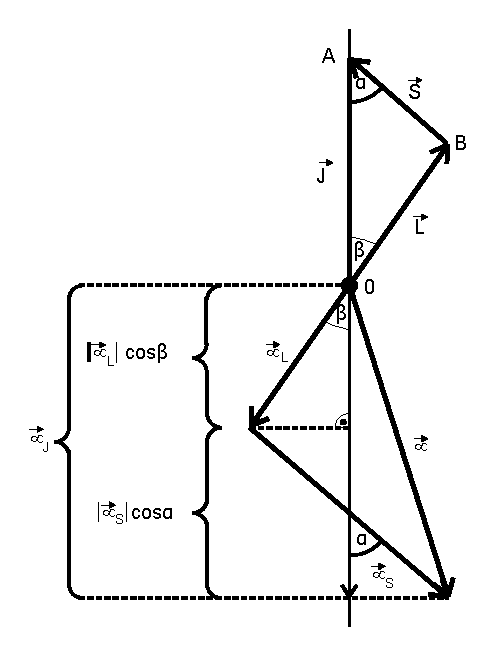
\includegraphics[width= 0.4 \linewidth]{pictures/Zeichnung1.pdf}
    \caption{Vektordiagramm der Drehimpulsvektoren einer Elektronenhülle und den daraus resultierenden magnetischen Momenten \cite{v606}.}
    \label{fig:Zeichnung1}
\end{figure}
Der Gesamtdrehimpuls $\vec{J}$ setzt sich aus drei Anteilen zusammen, welche auch schematisch in \autoref{fig:Zeichnung1} dargestellt sind.
Einmal der Bahndrehimpuls der Elektronenhülle, dem Eigendrehimpuls der Elektronen, auch Spin genannt, und der Kerndrehimpuls.
Letzterer kann hier vernachlässigt werden.
Es folgt also
\begin{equation}
    \vec{J} = \vec{L} + \vec{S},
\end{equation}
wobei $\vec{L}$ und $\vec{S}$ jeweils die Vektorsummen der Einzeldrehimpulse der Elektronen in der Hülle sind.
Quantenmechanisch lässt sich jetzt zeigen, dass
\begin{align}
    \vec{\mu_L} &= - \frac{\vec{\mu_B}}{\hbar} \vec{L} \quad \text{und} \\
    \vec{\mu_S} &= - \text{g}_S \frac{\vec{\mu_B}}{\hbar} \vec{S}
\end{align}
ist.
Dabei ist $\vec{\mu_B}$ das Bohrsche Magneton und $\text{g}_S$ das gyromagnetische Verhältnis des freien Elektrons.
Interessant sind oft die Beträge.
Mit
\begin{equation*}
    \left| \vec{J}\right| = \sqrt{J \left( J + 1 \right)} \cdot \hbar
\end{equation*}
folgt 
\begin{align}
    \left|\vec{\mu_L} \right| &= \mu_B \sqrt{L \left( L + 1 \right)} \\
    &\text{und} \nonumber \\
    \left|\vec{\mu_S} \right| &= \text{g}_S \mu_B \sqrt{S \left( S + 1 \right)}.
\end{align}
Durch einige geometrischen Beziehungen die sich aus \autoref{fig:Zeichnung1} entnehmen lassen und der Näherung von $\text{g}_S \approx 2$ folgt dann schließlich, dass
\begin{equation}
    \left|\vec{\mu}_{\mathrm{J}}\right| \approx \mu_{\mathrm{B}} \sqrt{\mathrm{J}(\mathrm{J}+1)} \frac{3 \mathrm{~J}(\mathrm{~J}+1)+\{\mathrm{S}(\mathrm{S}+1)-\mathrm{L}(\mathrm{L}+1)\}}{2 \mathrm{~J}(\mathrm{~J}+1)} .
\end{equation}
Dabei wird der Term
\begin{equation}
    g_{J}:=\frac{3 \mathrm{~J}(\mathrm{~J}+1)+\{\mathrm{S}(\mathrm{S}+1)-\mathrm{L}(\mathrm{L}+1)\}}{2 \mathrm{~J}(\mathrm{~J}+1)}
\end{equation}
der Landé-Faktor des betreffenden Atoms genannt. Damit gilt
\begin{equation}
    \left|\vec{\mu}_{\mathrm{J}}\right| \approx \mu_{\mathrm{B}} \mathrm{g}_{\mathrm{J}} \sqrt{\mathrm{J}(\mathrm{J}+1)}.
\end{equation}
Durch das quantenmechanische Phänomen der Richtungsquantelung gilt
\begin{equation}
    \mu_{J_z} = - \mu_B \text{g}_J m,
\end{equation}
wobei $m$ die Orientierungszahl ist.
Es lässt sich nun durch längere Rechnung zeigen, dass
\begin{equation}
    \chi=\frac{\mu_{0} \mu_{\mathrm{B}}^{2} \mathrm{~g}_{\mathrm{J}}^{2} \mathrm{NJ}(\mathrm{J}+1)}{3 \mathrm{kT}}
\end{equation}
ist \cite{v606}.
Dabei ist $N$ die Anzahl der Momente pro Volumeneinheit und $k$ die Boltzmann-Konstante.
Es lässt sich auch das Curiesche Gesetz des Paramagnetismus
\begin{equation}
    \chi \sim \frac{1}{T}
\end{equation}
erkennen.

Bekanntermaßen lässt sich Paramagnetismus sehr gut bei Verbindungen beobachten, die Ionen Seltener Erden enthalten.
Daraus lässt sich nach obigen Eigenschaften des Paramagnetismus folgern, dass die Elektronenhüllen dieser Verbindungen große Drehimpulse haben müssen.
Diese können nur durch die inneren Elektronen erzeugt werden, genauer gesagt durch die Elektronen in der 4f-Schale.
Die Anordnung der Elektronen in dieser Schale und der daraus resultierende Gesamtdrehimpuls $\vec{J}$ werden durch die sogenannten Hundschen Regeln beschrieben.
Diese lauten:
\begin{enumerate}
    \item Die Spins $\vec{s_i}$ kombinieren zum Gesamtspin $\vec{S} = \sum \vec{s_i}$ , die nach dem Pauli-Prinzip gebildet werden können
    \item Der maximale Drehimpuls $\vec{L} = \sum \vec{l_i}$ entsteht so, dass die Bahndrehimpulse $\vec{l_i}$ mit dem Pauli-Prinzip und der ersten Regel verträglich sind.
    \item Der Gesamtdrehimpuls ist $\vec{J} = \vec{L} - \vec{S}$, falls die Schale weniger als zu Hälfte gefüllt ist und $\vec{J} = \vec{L} + \vec{S}$, wenn sie mehr als zur Hälfte gefüllt ist.
\end{enumerate}

Diese Regeln basieren darauf, dass die Hüllenelektronen sich untereinander elektrostatisch abstoßen.


\subsection{Vorgehen zur Bestimmung der Suszeptibilität}
\begin{wrapfigure}{r}{0.4\linewidth}
    \center
    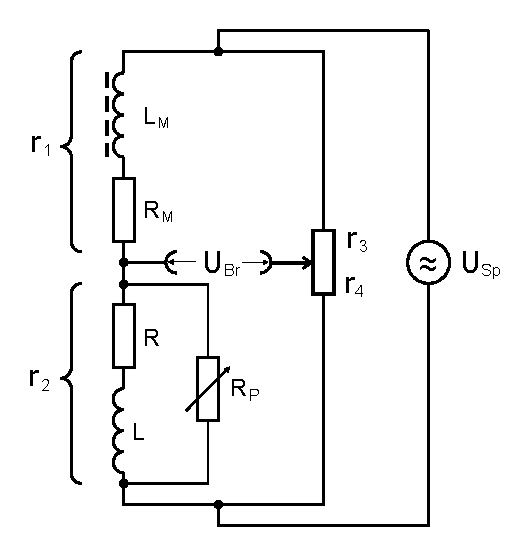
\includegraphics[width=\linewidth]{pictures/Zeichnung2.pdf}
    \caption{Suszeptibilitätsmessung mittels einer Brückenschaltung \cite{v606}.}
    \label{fig:Zeichnung2}
\end{wrapfigure}
Um die Suszeptibilität $\chi$ experimentell zu bestimmen, wird eine Brückenschaltung wie in \autoref{fig:Zeichnung2} verwendet.
Die Induktivität einer Spule ist durch
\begin{equation}
    L_\text{ges} = \mu \mu_0 \frac{n^2}{I} F
\end{equation}
gegeben, welche sich aber aufgrund der technischen Realisierbarkeit zu
\begin{equation}
    L_\text{ges} ' = \mu_0 \frac{n^2}{I} F + \chi \mu_0 \mu_0 \frac{n^2}{I} Q
\end{equation}
abändert. Dabei ist $Q$ der Querschnitt der Probe und $F$ der Spulenquerschnitt.
Es werden zwei Spulen möglichst gleicher Induktivität $L$ benutzt, da die Induktionsdifferenz $\increment L$ für die Suszeptibilitätsmessung entscheidend ist.
Nach langer Rechnung lässt sich für den hohe Frequenzen zeigen, dass
\begin{equation}
    \omega \rightarrow \inf: \chi = 2 \cdot \frac{\increment R}{R_3} \frac{F}{Q}
\end{equation}
gilt.
$R_3$ ist dabei der Widerstand am Potentiometer in \autoref{fig:Zeichnung2} und $\increment$ die Differenz am Potentiometer.